%%=============================================================================

\documentclass[10pt, aspectratio=169, 
    serif, mathserif, professionalfont, table, svgnames]{beamer}

%%-----------------------------------------------------------------------------
%% Incluídos pelo knitr.

\usepackage[]{graphicx}
\usepackage[]{color}
%% maxwidth is the original width if it is less than linewidth
%% otherwise use linewidth (to make sure the graphics do not exceed the margin)
\makeatletter
\def\maxwidth{ %
  \ifdim\Gin@nat@width>\linewidth
  \linewidth
  \else
  \Gin@nat@width
  \fi
}
\makeatother

\definecolor{fgcolor}{rgb}{0.345, 0.345, 0.345}
%\definecolor{fgcolor}{rgb}{0.5, 0.5, 0.5}
\newcommand{\hlnum}[1]{\textcolor[rgb]{0.686,0.059,0.569}{#1}}%
\newcommand{\hlstr}[1]{\textcolor[rgb]{0.192,0.494,0.8}{#1}}%
\newcommand{\hlcom}[1]{\textcolor[rgb]{0.678,0.584,0.686}{\textit{#1}}}%
\newcommand{\hlopt}[1]{\textcolor[rgb]{0,0,0}{#1}}%
\newcommand{\hlstd}[1]{\textcolor[rgb]{0.345,0.345,0.345}{#1}}%
\newcommand{\hlkwa}[1]{\textcolor[rgb]{0.161,0.373,0.58}{\textbf{#1}}}%
\newcommand{\hlkwb}[1]{\textcolor[rgb]{0.69,0.353,0.396}{#1}}%
\newcommand{\hlkwc}[1]{\textcolor[rgb]{0.333,0.667,0.333}{#1}}%
\newcommand{\hlkwd}[1]{\textcolor[rgb]{0.737,0.353,0.396}{\textbf{#1}}}%

\usepackage{framed}
\makeatletter
\newenvironment{kframe}{%
  \def\at@end@of@kframe{}%
  \ifinner\ifhmode%
  \def\at@end@of@kframe{\end{minipage}}%
\begin{minipage}{\columnwidth}%
  \fi\fi%
  \def\FrameCommand##1{\hskip\@totalleftmargin \hskip-\fboxsep
    \colorbox{shadecolor}{##1}\hskip-\fboxsep
    % There is no \\@totalrightmargin, so:
    \hskip-\linewidth \hskip-\@totalleftmargin \hskip\columnwidth}%
  \MakeFramed {\advance\hsize-\width
    \@totalleftmargin\z@ \linewidth\hsize
    \@setminipage}}%
{\par\unskip\endMakeFramed%
  \at@end@of@kframe}
\makeatother

\definecolor{shadecolor}{rgb}{.97, .97, .97}
\definecolor{messagecolor}{rgb}{0, 0, 0}
\definecolor{warningcolor}{rgb}{1, 0, 1}
\definecolor{errorcolor}{rgb}{1, 0, 0}
\newenvironment{knitrout}{}{} % an empty environment to be redefined in TeX

\usepackage{alltt}

%% Tamanho de fonte e distância entre linhas.
\renewenvironment{knitrout}{
  \footnotesize\renewcommand{\baselinestretch}{0.75}
}{}

%%-----------------------------------------------------------------------------
%% Pacotes padrões.

%% Fontes.
\usepackage{palatino}
\usepackage{eulervm}
\usepackage[none]{ubuntu}
\renewcommand{\ttdefault}{ubuntumono}
\renewcommand{\ttfamily}{\fontUbuntuMono}

%% Verbatim na fonte Ubuntu Mono.
\usepackage{verbatim}
\makeatletter
\def\verbatim@font{\small\fontUbuntuMono}
\makeatother

% Esses pacotes dão clash.
% http://tex.stackexchange.com/questions/51488/option-clash-with-xcolor-and-tikz
\usepackage{xcolor} %% opções no \documentclass{} para evitar clash.
\definecolor{mycolor}{rgb}{0.13,0.53,0.53}
\definecolor{mycolor2}{rgb}{0.725,0,0.18}

% http://tex.stackexchange.com/questions/50747/options-for-appearance-of-links-in-hyperref
\usepackage{hyperref}
\hypersetup{colorlinks, allcolors=.,
  urlcolor=mycolor2, runcolor=orange}

\usepackage[brazil]{babel}
\usepackage[utf8]{inputenc}
\usepackage{graphicx}
\usepackage{amsmath, amsfonts, amssymb, amsxtra, amsthm, icomma}
\usepackage{geometry, calc, setspace, indentfirst}
\usepackage{multicol, multirow}
\usepackage{pbox}
\usepackage{colortbl}
\usepackage{booktabs} % \toprule, \midrule and \bottomrule em tabelas.
\usepackage{enumerate}
% \usepackage{paralist} %% compact{item,enum}. Não usar em beamer.
\usepackage{float}
\usepackage[hang]{caption}
\captionsetup{font=footnotesize, labelfont=footnotesize, labelsep=period}
\usepackage{fancybox}
\usepackage{fancyvrb} %% Permite vebatim dentro de fbox{}.

%% Texto no corpo do beamer justificado.
\usepackage{ragged2e}
\justifying

%%-----------------------------------------------------------------------------

%% A lot of options: http://latex-community.org/forum/viewtopic.php?f=55&t=17646
\useoutertheme[width=60pt, height=30pt, right, hideothersubsections]{sidebar}
\setbeamercolor{structure}{fg=mycolor}

\makeatletter
\setbeamertemplate{section in toc}[sections numbered]
\setbeamertemplate{subsection in toc}[subsections numbered]
\setbeamertemplate{sections/subsections in toc}[ball]{}
\setbeamertemplate{section in sidebar right}[sections numbered]

%% http://tex.stackexchange.com/questions/250836/reduce-fontsize-beamer-sidebar
\setbeamerfont{title in sidebar}{size=\fontsize{6}{1}\selectfont}
\setbeamerfont{section in sidebar}{size=\fontsize{6}{7}\selectfont}
\setbeamerfont{subsection in sidebar}{size=\fontsize{5}{5}\selectfont}

\setbeamertemplate{caption}[numbered]
\setbeamertemplate{frametitle continuation}{\gdef\beamer@frametitle{}}
\setbeamertemplate{navigation symbols}{} %% Retira a barra de navegação.
% \setbeamertemplate{blocks}[rounded][shadow=FALSE]
% \setbeamercolor{block title}{fg=structure, bg=mycolor!20!white}
\makeatother

% http://tex.stackexchange.com/questions/109816/automatic-frame-titles-subtitles-with-condition
\makeatletter
\CheckCommand*\beamer@checkframetitle{%
  \@ifnextchar\bgroup\beamer@inlineframetitle{}}
\renewcommand*\beamer@checkframetitle{%
  \global\let\beamer@frametitle\relax\@ifnextchar%
  \bgroup\beamer@inlineframetitle{}}
\makeatother

\addtobeamertemplate{frametitle}{
  \ifx\insertframetitle\empty
    \ifx\insertframesubtitle\empty
      \ifx\insertsubsection\empty 
        \frametitle{\insertsectionhead}
      \else
        \frametitle{\insertsubsectionhead}\framesubtitle{\insertsectionhead}
      \fi  
    \else     
    \fi  
  \else
  \fi
}{}

%%-----------------------------------------------------------------------------

% \usebackgroundtemplate{
%   \includegraphics[width=\paperwidth]{./images/ufpr_bg3.jpg}
% }

\AtBeginSection[]{
  \begin{frame}[c, allowframebreaks]
    \frametitle{\phantom{1}}
    \framesubtitle{\phantom{1}}
    \begin{center}
      \textcolor{mycolor}{\thesection} \\ \vspace{0.3cm}
      \parbox{0.6\textwidth}{
        \centering \textcolor{mycolor}{\LARGE \insertsection}}\\
    \end{center}
  \end{frame}
}

%% Spacing between items (itemize)
\let\olditem\item
\renewcommand{\item}{%
  \olditem\vspace{6pt}}

%%-----------------------------------------------------------------------------
%% Definições dos proprietários.

\title[Explorando interfaces gráficas com o R]{\LARGE Explorando interfaces gráficas com o R}
\author[]{\small
  Prof. Dr. Walmes M. Zeviani\\
  Eduardo E. Ribeiro Jr\\ 
  Vanessa F. Sehaber\\
  Karina B. Rebuli\\
  Henrique A. Laureano
}

\institute[UFPR]{
  Laboratório de Estatística e Geoinformação \\
  Programa de Educação Tutorial\\
  Departamento de Estatística \\
  Universidade Federal do Paraná}
\date{}
\logo{
\includegraphics[width=1.4cm]{./images/ufpr_logo.jpg}}

%%=============================================================================

\begin{document}

%\begin{comment}
\frame{
  \vspace{-1.0cm}
  \titlepage
  \vspace{-1.6cm}
  \begin{center}
    % \includegraphics[width=4.0cm]{./images/leg2.png}\\
    \href{http://www.leg.ufpr.br}{www.leg.ufpr.br}\\
	%\href{http://www.pet.est.ufpr.br}{www.leg.ufpr.br}\\    
	\texttt{walmes@ufpr.br}
  \end{center}
}

\begin{frame}{Disponibilização}

  \begin{minipage}[c]{0.1\linewidth}
    \begin{center}	
      
\includegraphics[scale=0.07]{./images/github_icon}\\
      \vspace{0.3cm}
    \end{center}
  \end{minipage}
  \hfill % Final de fig1 e inicio de fig2
  \begin{minipage}[c]{0.85\linewidth}
    % \href{https://github.com/JrEduardo/iguiR}{\texttt{https://github.com/JrEduardo/iguiR}}
    \texttt{\url{https://github.com/JrEduardo/iguiR}} (sujeito a atualização)\\
    \texttt{\url{http://www.leg.ufpr.br/iguiR}} (zip da versão de hoje)
  \end{minipage}

  \vspace{0.3cm}
  {\tt
    \textcolor{mycolor2}{I}nteractive
    \textcolor{mycolor2}{G}raphical
    \textcolor{mycolor2}{U}ser
    \textcolor{mycolor2}{I}nterface in
    \textcolor{mycolor2}{R} -
  }\href{https://github.com/JrEduardo/iguiR}{\texttt{iguiR}}\\
  
\end{frame}

%\end{comment}

%%=============================================================================

\section{Introdução}

\subsection{Motivação}

\begin{frame}

  \begin{minipage}[c]{0.8\linewidth}
    \begin{center}
      \it Se uma imagem vale mais que 1000 palavras então\ldots
      \pause~\\
      um recurso interativo vale mais que 1000 imagens.
    \end{center}
  \end{minipage}
  \vspace{2em}

  \begin{multicols}{2}
    \pause
    \begin{block}{Objetivo}
      Apresentar ferramentas para facilitar
      \begin{enumerate}
        \itemsep-2pt\parskip0pt\parsep0pt
      \item a compreensão de conceitos/resultados,
      \item a realização de tarefas e
      \item como compartilhar esses recursos.
      \end{enumerate}
    \end{block}
    \vfill
    \columnbreak
    \pause
    \begin{block}{Uso em potencial}
      \begin{itemize}
      \item como instrumento de ensino,
      \item para construir mini aplicativos e
      \item para produzir relatórios/aplicações web interativos.
      \end{itemize}
    \end{block}
  \end{multicols}
\end{frame}

\begin{frame}

  \begin{block}{Nossa experiência}
    \begin{itemize}
    \item Animações para matérias de blog;
    \item Instrumento de ensino em material online;
    \item Aplicação para ajuste de modelos não lineares;
    \item Aplicações para ensino de Estatística;
    \item O Grupo PET Estatística desenvolveu várias aplicações para
      feira de profissões;
    \item Discentes criam a Academia de Estatística Computacional e Programação;
    \item Aquisição da servidora RStudio/Shiny do LEG \& PET;
    \item Crescente demanda de recursos para visualização de dados espaço
      temporais.
    \end{itemize}
  \end{block}

\end{frame}

\subsection{Conteúdo}

\begin{frame}
\vspace{-1.0cm}

\begin{columns}[t]
\begin{column}{.3\textwidth}
  \vspace{1cm}
  \begin{block}{Recursos interativos}
    \begin{itemize}
      \setbeamercovered{transparent=35}
      \uncover<2>{\item \texttt{animation}}
      \uncover<3>{\item \texttt{rgl}}
      \uncover<4>{\item \texttt{googleVis}}
      \uncover<5>{\item \texttt{gWidgets}}
      \uncover<6>{\item \texttt{rpanel}}
      \uncover<7>{\item \texttt{shiny}}
    \end{itemize}
  \end{block}
  \vspace{1cm}
\end{column}

\begin{column}{.6\textwidth}
  \vspace{0.5cm}
  \only<2>{
    {\center
      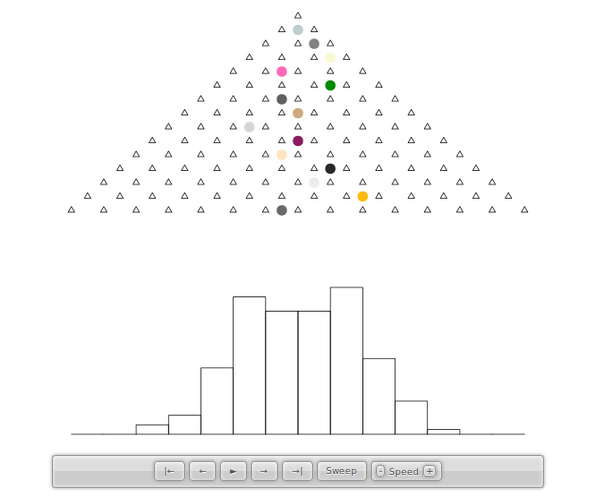
\includegraphics[scale=0.3]{images/preview_ani}}}
  \only<3>{
    {\center
      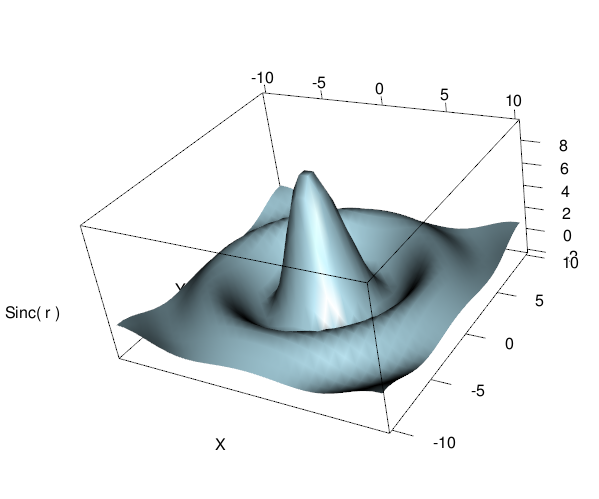
\includegraphics[scale=0.3]{images/preview_rgl}}}
  \only<4>{
    {\center 
      \vspace{-0.7cm}
      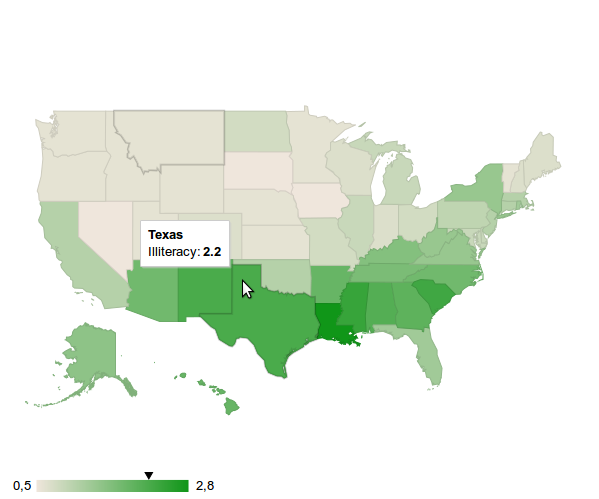
\includegraphics[scale=0.3]{images/preview_ggvis}}}
  \only<5>{
    {\center
      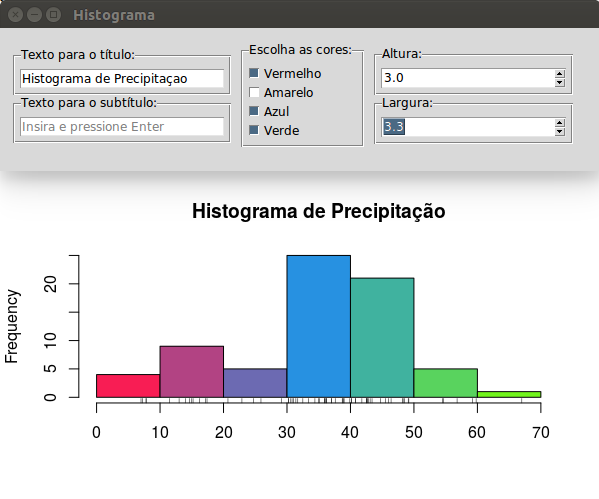
\includegraphics[scale=0.3]{images/preview_gwidgets}}}
  \only<6>{
    {\center
      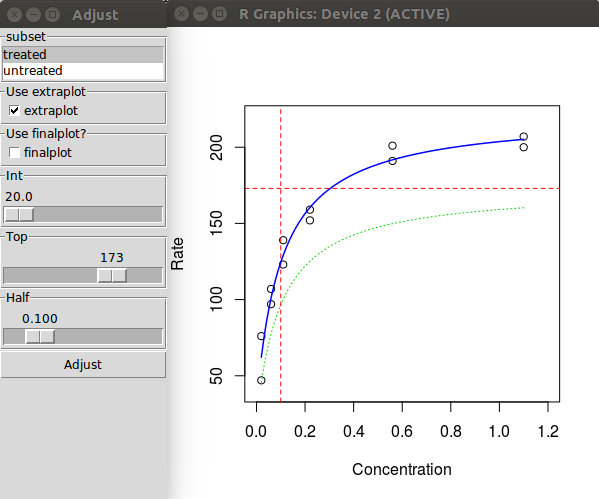
\includegraphics[scale=0.3]{images/preview_rpanel}}}
  \only<7>{
    {\center
      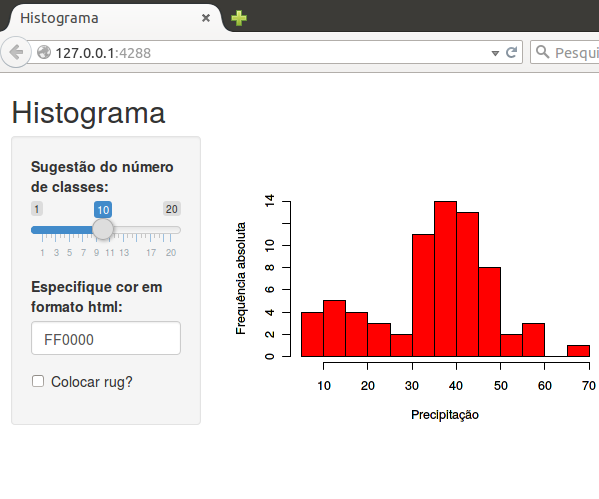
\includegraphics[scale=0.3]{images/preview_shiny}}}
  \end{column}
\end{columns}

\end{frame}


\begin{frame}{Conteúdo}
  \begin{multicols}{2}
    \small{\tableofcontents}
  \end{multicols}
\end{frame}

\section{\texttt{animation}}

%----------------------------------------------------------------------

\subsection{Descrição}

\begin{frame}

  \texttt{animation} contém uma variedade de funções para produzir
  animações com o R. As animações podem ser produzidas em vários
  formatos: flash, gif, html, pdf e vídeos.

  \begin{itemize}
    \itemsep1pt\parskip0pt\parsep0pt
  \item Autores: Yihui Xie, Lijia Yu, Weicheng Zhu
  \item Lançamento: 11-Nov-2007
  \item Versão: 2.3
  \item URL:
    \url{http://cran.r-project.org/web/packages/animation/index.html},
    \url{http://yihui.name/animation/}
  \end{itemize}

\end{frame}

%----------------------------------------------------------------------

\subsection{Como usar}

\begin{frame}

  modelo característico.

\end{frame}

%----------------------------------------------------------------------

\subsection{Exemplos}

\begin{frame}

  links para executáveis e galerias.

  Algumas aplicações com o animation:
  \begin{itemize}
    \itemsep1pt\parskip0pt\parsep0pt
  \item
    \href{http://vis.supstat.com/categories.html\#animation-ref}{Galeria
      do autor},
  \item \href{http://www.r-bloggers.com/?s=animation}{Busca no R
      Bloggers},
  \end{itemize}

\end{frame}
\section{\texttt{rgl}}

\subsection*{Descrição}

%----------------------------------------------------------------------

\begin{frame}

  \texttt{rgl} oferece funções de médio a alto nível para gráficos 3D
  interativos, tanto as representações em 3D de gráficos simples em 2D
  quanto para representações objetos geométricos no espaço (cubos,
  elipses, etc). A visualização pode ser na tela com OpenGL ou em outros
  formados como WebGL.

  \begin{itemize}
  \item Autores: Daniel Adler, Duncan Murdoch, e outros
  \item Lançamento: 04-Mar-2004
  \item Versão: 0.95.1247
  \item URL: \url{http://cran.r-project.org/web/packages/rgl/index.html}
  \item Algumas aplicações com o \texttt{rgl}:

  \begin{itemize}
    \itemsep1pt\parskip0pt\parsep0pt
  \item \href{http://www.r-bloggers.com/?s=rgl}{Busca no R Bloggers}
  \end{itemize}
\end{itemize}

\end{frame}

%----------------------------------------------------------------------

\subsection*{Como usar}

\begin{frame}

\vspace{-1.0cm}
\setlength{\columnsep}{5pt}
\begin{multicols}{2}
\begin{knitrout}\footnotesize
\definecolor{shadecolor}{rgb}{0.969, 0.969, 0.969}\color{fgcolor}\begin{kframe}
\begin{alltt}
\hlkwd{require}\hlstd{(graphics)}

\hlkwd{plot}\hlstd{(...)}
\hlkwd{persp}\hlstd{(...)}
\hlkwd{abline}\hlstd{(...)}
\hlkwd{box}\hlstd{(...)}
\hlkwd{legend}\hlstd{(...)}
\hlkwd{text}\hlstd{(...)}
\hlkwd{points}\hlstd{(...)}
\hlkwd{lines}\hlstd{(...)}
\hlkwd{segments}\hlstd{(...)}
\hlkwd{mtext}\hlstd{(...)}
\hlkwd{par}\hlstd{(}\hlkwc{mfrow}\hlstd{= ...)}
\hlstd{...}
\end{alltt}
\end{kframe}
\end{knitrout}

\begin{knitrout}\footnotesize
\definecolor{shadecolor}{rgb}{0.969, 0.969, 0.969}\color{fgcolor}\begin{kframe}
\begin{alltt}
\hlkwd{require}\hlstd{(rgl)}

\hlkwd{plot3d}\hlstd{(...)}
\hlkwd{persp3d}\hlstd{(...)}
\hlkwd{abclines3d}\hlstd{(...)}
\hlkwd{box3d}\hlstd{(...)}
\hlkwd{legend3d}\hlstd{(...)}
\hlkwd{text3d}\hlstd{(...)}
\hlkwd{points3d}\hlstd{(...)}
\hlkwd{lines3d}\hlstd{(...)}
\hlkwd{segments3d}\hlstd{(...)}
\hlkwd{mtext3d}\hlstd{(...)}
\hlkwd{mfrow3d}\hlstd{(...)}
\hlstd{...}
\end{alltt}
\end{kframe}
\end{knitrout}
\end{multicols}

\pause
\vspace{-0.6cm}
\begin{knitrout}\footnotesize
\definecolor{shadecolor}{rgb}{0.969, 0.969, 0.969}\color{fgcolor}\begin{kframe}
\begin{alltt}
\hlkwd{snapshot3d}\hlstd{(}\hlkwc{filename}\hlstd{=}\hlstr{"fig3d"}\hlstd{)}

\hlkwd{rgl.postscript}\hlstd{(}\hlstr{"fig3d.pdf"}\hlstd{,}
               \hlstr{"pdf"}\hlstd{,}
               \hlkwc{drawText}\hlstd{=}\hlnum{FALSE}\hlstd{)}

\hlkwd{writeWebGL}\hlstd{(...)}
\end{alltt}
\end{kframe}
\end{knitrout}


\end{frame}

%----------------------------------------------------------------------

\subsection*{Exemplos}

\begin{frame}

 Praticando:
  \begin{enumerate}
  \item
    \href{run:./R/rgl/rgl.R}{R Script rgl}
  \item 
	\href{run:./rgl/RGL.html}{Galeria rgl IGUIR}
  \end{enumerate}

  \vspace{0.5cm}
  Algumas aplicações com o rgl:
  \begin{itemize}
  \item \href{http://cran.r-project.org/web/packages/rgl/vignettes/}{Galeria
      do autor},
  \item \href{http://www.r-bloggers.com/?s=rgl}{Busca no R
      Bloggers}
  \end{itemize}

\end{frame}

\section{\texttt{googleVis}}

%----------------------------------------------------------------------

\subsection{Descrição}

\begin{frame}

  Funções R para gráficos \textit{a la}
  \href{https://developers.google.com/chart/interactive/docs/gallery}{Google
    Docs SpreadSheets}.
  \vspace{2em}

  \begin{itemize}
  \item Autores: Markus Gesmann, Diego de Castillo, Joe Cheng
  \item Lançamento: 03-Dec-2010
  \item Versão: 0.5.9
  \item URL:
    \url{http://cran.r-project.org/web/packages/googleVis/index.html},
    \url{https://github.com/mages/googleVis}
  \end{itemize}
  
\end{frame}

\begin{frame}

  \begin{columns}
    \column{0.5\linewidth}
    \begin{itemize}
    \item O mais conhecido: \textbf{Motion Chart}, popularizado por Hans
      Rosling em seu
      \href{https://www.ted.com/talks/hans_rosling_shows_the_best_stats_you_ve_ever_seen}{TED
        talk}.
    \item Visualizar dados em data frames com gráficos Google sem upload
      no Google Docs.
    \item O resultado é um html com funções JavaScript hopedadas pelo
      Google que é rederizado pelo navegador.
    \item Requer conexão, às vezes flash.
    \end{itemize}

    \column{0.49\linewidth}
    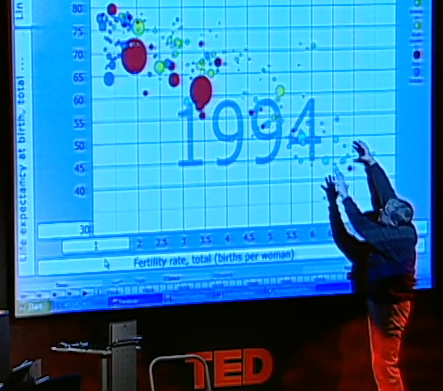
\includegraphics[width=\linewidth]{./images/ted-hans-hosling.png}
  \end{columns}

\end{frame}

\begin{frame}
  \begin{itemize}
  \item Dado estruturado em \texttt{DataTable}.
  \item Transforma \texttt{data.frame}s em objetos JSON.
  \item Usa o \texttt{RJSONIO} para gerar JSON.
  \end{itemize}

  \begin{center}
    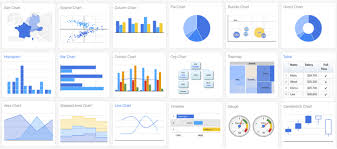
\includegraphics[width=0.5\linewidth]{./images/googleVis.jpg}
  \end{center}

\end{frame}

%----------------------------------------------------------------------

\subsection{Como usar}
  
\frame{
  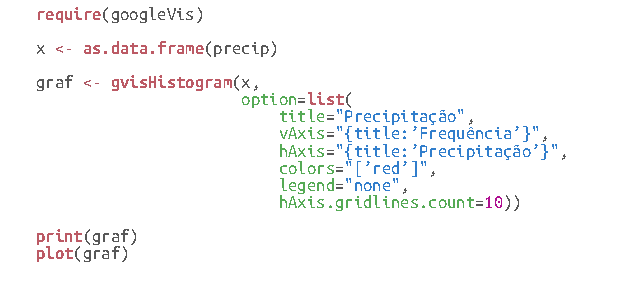
\includegraphics{./tikz/googleVis_gvisHistogram-1.pdf}
}  

\frame{
  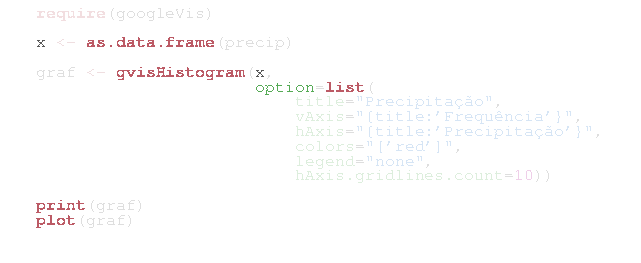
\includegraphics{./tikz/googleVis_gvisHistogram-2.pdf}
}

\frame{
  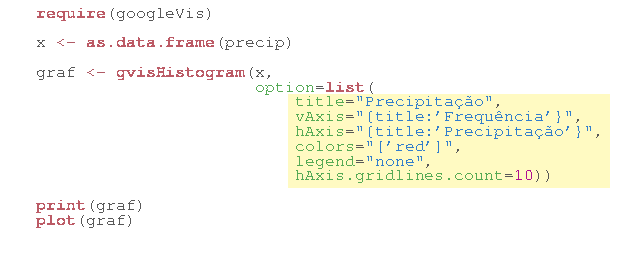
\includegraphics{./tikz/googleVis_gvisHistogram-3.pdf}
}

%----------------------------------------------------------------------

\subsection{Exemplos}

\begin{frame}

 Praticando:
  \begin{enumerate}
  \item \href{run:./R/googleVis/googleVis.R}{R Script googleVis}
  \end{enumerate}

  \vspace{0.5cm}
  Algumas aplicações com o googleVis:
  \begin{itemize}
  \item \href{http://cran.r-project.org/web/packages/googleVis/vignettes/}{Galeria
      do autor}
  \item \href{http://www.r-bloggers.com/?s=googleVis}{Busca no R
      Bloggers}
  \end{itemize}

\end{frame}

\section{\texttt{gWidgets}}

%----------------------------------------------------------------------

\subsection{Descrição}

\begin{frame}

  \texttt{gWidgets} fornece um kit de ferramentas para construir
  interfaces gráficas interativas.

  \vspace{\baselineskip}

  Verzani, M., Lawrence, M. (2012). \emph{Programming Graphical User
    Interfaces in R}, CRC Press.

  \begin{itemize}
  \item Autor: John Verzani
  \item Lançamento: 29-Sep-2006
  \item Versão: 0.0-54
  \item URL: \url{http://cran.r-project.org/web/packages/gWidgets/index.html}
  \end{itemize}

\end{frame}

\begin{frame}

  \begin{itemize}
  \item Alguns pacotes baseados em toolkits suportadas:
    \begin{itemize}
    \item tcl/tk:
      \href{http://cran.r-project.org/web/packages/gWidgetstcltk/index.html}{\texttt{gWidgetstcltk}}
      \href{http://cran.r-project.org/web/packages/Rcmdr/index.html}{\texttt{Rcmdr}},
      \href{http://cran.r-project.org/web/packages/TeachingDemos/index.html}{\texttt{TeachingDemos}},
      \href{http://cran.r-project.org/web/packages/MetSizeR/index.html}{\texttt{MetSizeR}},
      \href{http://cran.r-project.org/web/packages/MergeGUI/index.html}{\texttt{MergeGUI}},
      \href{http://cran.r-project.org/web/packages/GrapheR/index.html}{\texttt{GrapheR}},
      \href{http://cran.r-project.org/web/packages/BiplotGUI/index.html}{\texttt{BiplotGUI}},
      \href{http://cran.r-project.org/web/packages/TestScorer/index.html}{\texttt{TestScorer}}
      e muitos outros.
    \item gtk:
      \href{http://cran.r-project.org/web/packages/gWidgetsRGtk2/index.html}{\texttt{gWidgetsRGtk2}}
      \href{http://cran.r-project.org/web/packages/playwith/index.html}{\texttt{playwith}},
      \href{http://cran.r-project.org/web/packages/MissingDataGUI/index.html}{\texttt{MissingDataGUI}},
      \href{http://cran.r-project.org/web/packages/GroupSeq/index.html}{\texttt{GroupSeq}},
      \href{http://cran.r-project.org/web/packages/AtelieR/index.html}{\texttt{AtelieR}},
      \href{http://cran.r-project.org/web/packages/vmsbase/index.html}{\texttt{vmsbase}},
      \href{http://cran.r-project.org/web/packages/reshapeGUI/index.html}{\texttt{reshapeGUI}},
      \href{http://cran.r-project.org/web/packages/R2STATS/index.html}{\texttt{R2STATS}}
      e muitos outros.
  \end{itemize}
\end{itemize}

\end{frame}

%----------------------------------------------------------------------

\subsection{Como usar}

\begin{frame}

  modelo característico.

\end{frame}

%----------------------------------------------------------------------

\subsection{Exemplos}

\begin{frame}
  \begin{enumerate}
  \item \href{run:./tikz/code.Rnw}{code.Rnw}
  \item \href{./tikz/code.Rnw}{code.Rnw}
  \item \url{./tikz/code.Rnw}
  \item links para executáveis e galeria.
  \end{enumerate}
\end{frame}


\section{\texttt{rpanel}}

\subsection{Descrição}

%----------------------------------------------------------------------

\begin{frame}

  \texttt{rpanel} fornece um conjunto de funções para criar interfaces
  gráficas simples para controlar funções do R. Além destas, o pacote
  tem funções para interfaces específicas chamadas de \emph{cartoons}. É
  baseado em Tcl/Tk.

  \begin{itemize}
  \item Autores: Bowman, Bowman, Gibson and Crawford
  \item Lançamento: 21-Aug-2006
  \item Versão: 1.1-3
  \item URL:
    \url{http://cran.r-project.org/web/packages/rpanel/index.html}
\end{itemize}

\end{frame}

%----------------------------------------------------------------------

\subsection{Como usar}

\frame{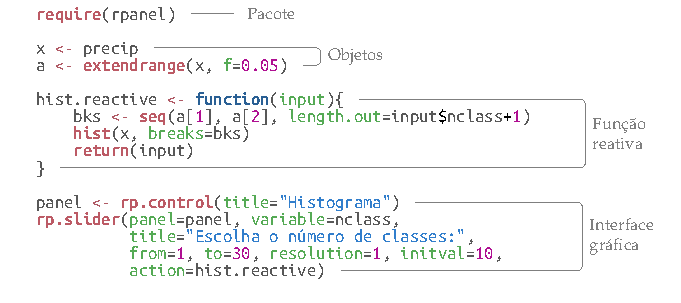
\includegraphics{./tikz/hist_slider_rpanel-1.pdf}}
\frame{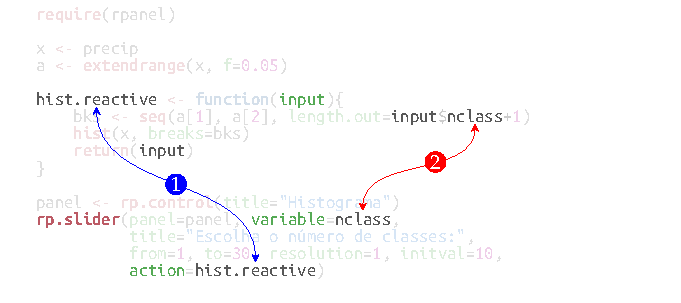
\includegraphics{./tikz/hist_slider_rpanel-2.pdf}}

\frame{
  \begin{center}
    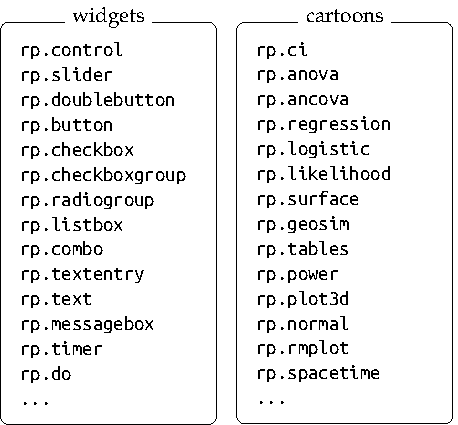
\includegraphics{./tikz/rpanel_fun.pdf}
  \end{center}
}

%----------------------------------------------------------------------

\subsection{Exemplos}

\begin{frame}
 Praticando:
  \begin{enumerate}
  \item
    \href{run:./R/rpanel/rpanel.R}{R Script rpanel}
  \item 
    \href{run:rpanel.html}{Galeria rpanel iguiR}
  \end{enumerate}

  \vspace{0.5cm}
  Algumas aplicações com o rpanel:
  \begin{itemize}
  \item \href{http://www.stats.gla.ac.uk/~adrian/rpanel/}{Galeria
      do autor}
  \item \href{http://www.r-bloggers.com/?s=rpanel}{Busca no R
      Bloggers}
  \end{itemize}

\end{frame}

\begin{frame}

  Alguns pacotes com GUI baseadas em \texttt{rpanel}:
  \begin{itemize}
  \item \href{http://cran.r-project.org/web/packages/GUIDE/index.html}{\texttt{GUIDE}}
  \item \href{http://cran.r-project.org/web/packages/MDSGUI/index.html}{\texttt{MDSGUI}}
  \item \href{http://cran.r-project.org/web/packages/RVideoPoker/index.html}{\texttt{RVideoPoker}}
  \item
    \href{https://github.com/walmes/wzRfun/blob/master/R/rp.nls.R}{\texttt{wzRfun::rp.nls}}
    (\href{run:./images/rp-nls.gif}{abrir gif}).
  \item \ldots
  \end{itemize}

\end{frame}

\section{\texttt{shiny}}

%----------------------------------------------------------------------

\subsection*{Descrição}

\begin{frame}

  \texttt{shiny} torna incrivelmente fácil construir aplicações web
  interativas com o R. Ligação entre \emph{inputs} e \emph{outputs} que
  são reativos e um conjunto extenso de \emph{widgets} permitem
  construir interfaces atraentes, responsivas e poderosas para a web com
  esforço mínimo.

  \begin{itemize}
  \item Autores: Winston Chang, Joe Cheng, JJ Allaire, Yihui Xie,
    Jonathan McPherson, e muitos contribuidores
  \item Lançamento: 01-Dec-2012
  \item Versão: 0.12.1
  \item URL:
    \url{http://cran.r-project.org/web/packages/shiny/index.html},
    \url{http://shiny.rstudio.com/}
  \end{itemize}

\end{frame}

%----------------------------------------------------------------------

\subsection*{Como usar}

\begin{frame}
  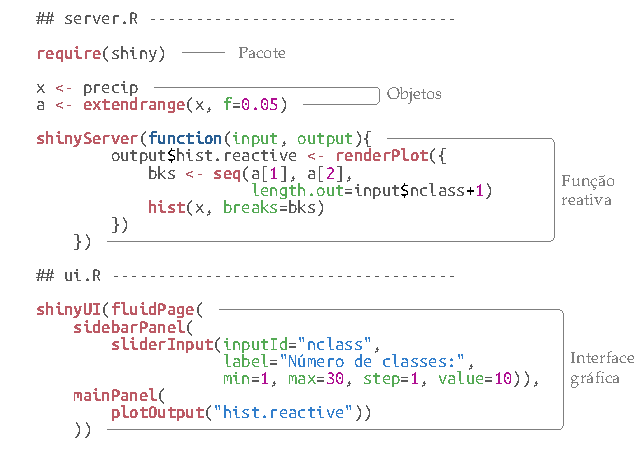
\includegraphics[scale=0.9]{./tikz/hist_slider_shiny-1.pdf}
\end{frame}

\begin{frame}
  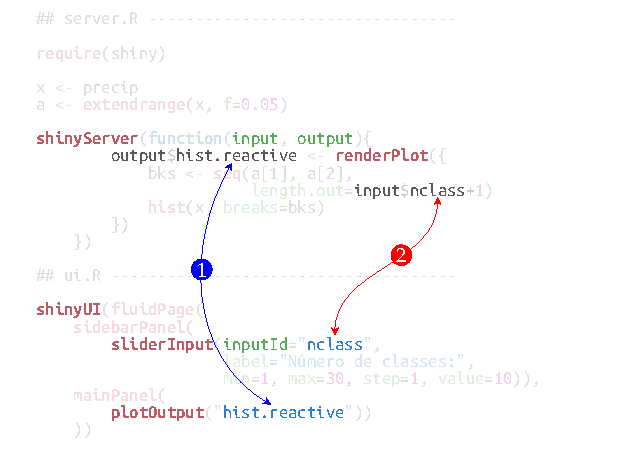
\includegraphics[scale=0.9]{./tikz/hist_slider_shiny-2.pdf}
\end{frame}

\frame{
  \begin{center}
    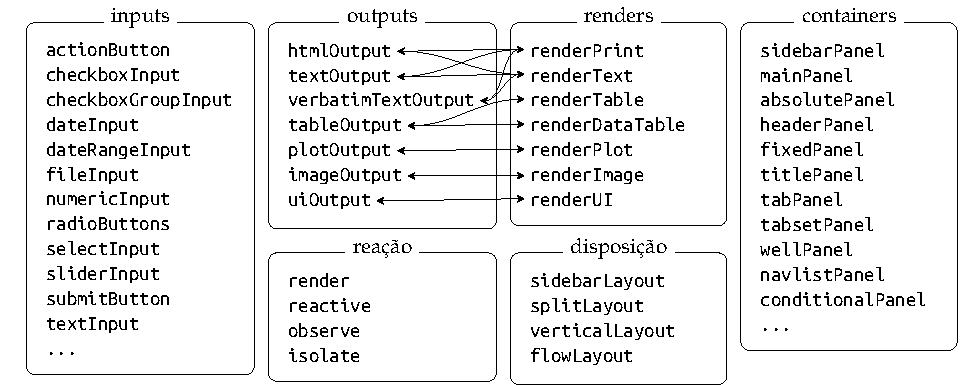
\includegraphics{./tikz/shiny_fun.pdf}
  \end{center}
}

\frame{
  \begin{center}
    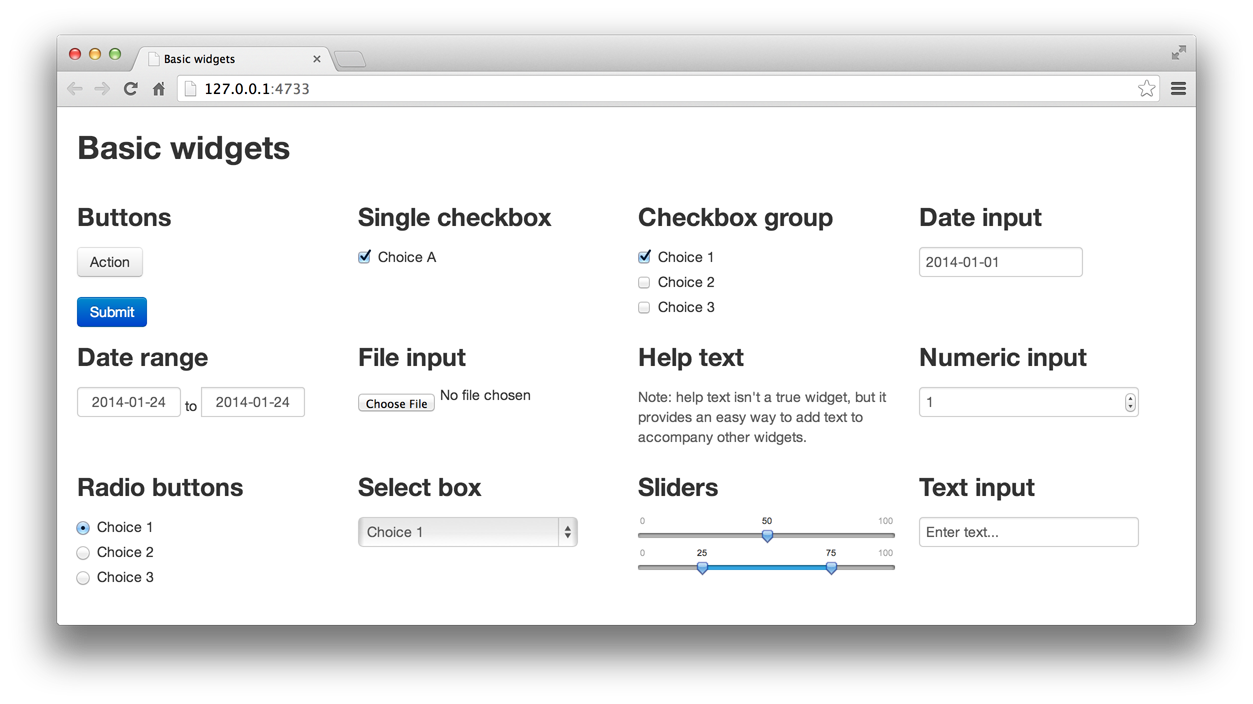
\includegraphics[width=0.9\linewidth]{./images/shiny-widgets.png}
  \end{center}
}

\frame{
  \begin{center}
    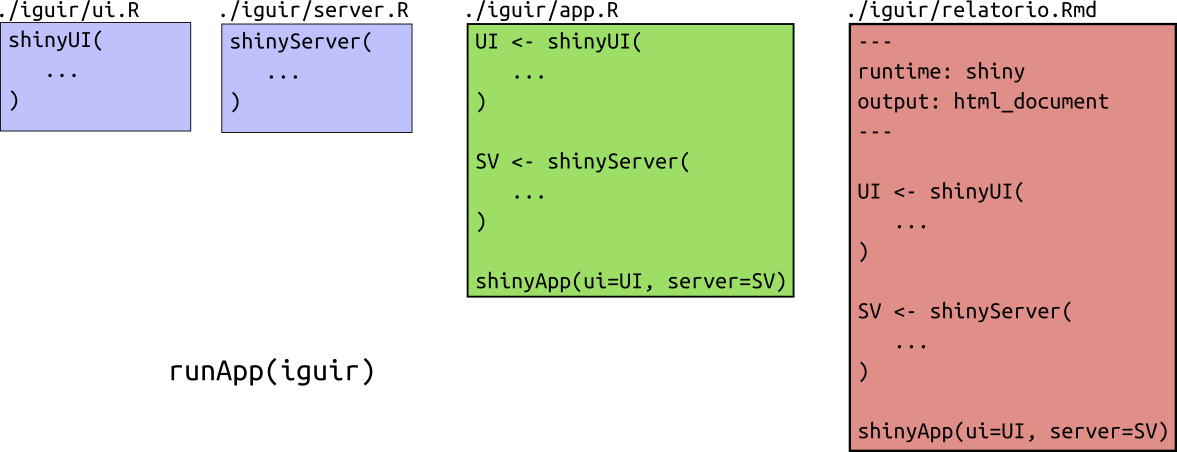
\includegraphics[width=0.9\linewidth]{./images/shiny_docs.png}
  \end{center}
}

\begin{frame}
  \begin{itemize}
  \item Criar aplicações com GUI (abrem no navegador);
  \item Produzir relatórios de análises web interativos;
  \item Não é necessário conhecimento de HTML, CSS ou JavaScript;
  \item Públicar aplicações na web
    \begin{itemize}
    \item \url{http://www.shinyapps.io/}
    \item Servidor Shiny próprio (\href{http://200.17.213.89:3838/iguir/list/}{Shiny LEG \& PET})
    \end{itemize}
  \item O público não precisa ter/saber o R.
  \end{itemize}
\end{frame}

%----------------------------------------------------------------------

\subsection*{Exemplos}

\begin{frame}
 Praticando:
  \begin{enumerate}
  \item \href{run:./R/shiny/shiny}{R Scripts shiny (sliderInput)}
  \item \href{run:./R/shiny/shiny2}{R Scripts shiny (radioButtons)}
  \end{enumerate}

  \vspace{0.5cm}
  Algumas galerias de aplicações em shiny:

  \begin{itemize}
  \item \href{http://200.17.213.89:3838/iguir/list/}{Galeria shiny
      IGUIR}
  \item \href{http://shiny.rstudio.com/gallery/}{Galeria Shiny Oficial}
  \item \href{http://www.showmeshiny.com/}{Galeria Shiny}
  \end{itemize}
  
\end{frame}

\begin{frame}
  Algumas aplicações em \texttt{shiny}:
  \begin{itemize}
  \item \href{http://www.stat.cmu.edu:3838/hseltman/LogReg/}{Logistic
      Regression Residual Analysis}
  \item \href{https://ilame.shinyapps.io/Test3}{Body Mass Index
      Calculation Tool}
  \item
    \href{https://hseltman.shinyapps.io/QuantileNormal}{Investigation of
      Quantile-Normal Plots Through Simulation}
  \item
    \href{http://www.stat.cmu.edu:3838/hseltman/PrePost/}{Pre-test/Post-test
      Simulation}
  \item
    \href{http://www.stat.cmu.edu:3838/hseltman/TransferFunctions/}{Explore
      Transfer Functions}
  \item
    \href{http://nbcgib.uesc.br/lec/avale-es/amb-virtual/inferencia/anava}{Fundamentos
      da análise de variância}
  \item
    \href{http://nbcgib.uesc.br/lec/avale-es/amb-virtual/probabilidade/con-frequentista}{Conceito
      frequentista de probabilidade}
  \end{itemize}

\end{frame}

\section{Ficaram de fora}

\begin{frame}

  \begin{itemize}
  \item 
    \href{https://cran.r-project.org/web/packages/manipulate/index.html}{\texttt{manipulate}}
  \item 
    \href{http://ramnathv.github.io/rCharts/}{\texttt{rCharts}}
  \item
    \href{http://cran.r-project.org/web/packages/iplots/index.html}{\texttt{iplots}}
  \item
    \href{http://cran.r-project.org/web/packages/rggobi/index.html}{\texttt{rggobi}}
  \item
    \href{https://rstudio.github.io/dygraphs/index.html}{\texttt{dygraphs}}
  \item
    \href{http://rstudio.github.io/shinydashboard/index.html}{\texttt{shinydashboard}}
  \item
    \href{https://cran.r-project.org/web/packages/gWidgets2/index.html}{\texttt{gWidgets2}}:
    \texttt{gWidgets2RGtk2}, \texttt{gWidgets2Qt} e \texttt{gWidgets2tcltk}.
  \item
    \href{http://www.htmlwidgets.org/index.html}{\texttt{htmlwidgets}}
  \end{itemize}

\end{frame}

\section{Considerações finais}

\begin{frame}

  \begin{multicols}{2}
    \begin{itemize}
    \pause \item Sem interação, apenas mudança de estados, resultado visual:
      \pause
      \begin{center}
        \texttt{animation}
      \end{center}
    \pause \item Explorar espaço 3D: \pause
      \begin{center}
        rgl
      \end{center}
      \pause \item Padrão Google Docs, edição e informações com eventos
      de mouse \pause
      \begin{center}
        googleVis
      \end{center}
      \vfill \columnbreak
    \pause \item Aplicação local de GUI pequena: \pause
      \begin{center}
        rpanel
      \end{center}
    \pause \item Aplicação local de GUI média, com mais \textit{handlers} e
      layout: \pause
      \begin{center}
        gWidgets
      \end{center}
    \pause \item Aplicação para a web: \pause
      \begin{center}
        shiny
      \end{center}
    \end{itemize}
  \end{multicols}

\end{frame}

\section{Agradecimentos}

\begin{frame}

  \begin{itemize}
  \item À organização da RBRAS
  \item Ao LEG e ao PET
  \item Aos acadêmicos do Curso de Estatística
  \item À comunidade R e do software livre
  \item Ao Prof.~Dr.~Ivan Allaman (UESC)
  \end{itemize}

\end{frame}

\begin{frame}
  \frametitle{}
  \framesubtitle{}

  \begin{center}
    Colaboração
  \end{center}
  \begin{columns}[t]
    \column{0.45\textwidth}
    \hfill
\includegraphics[width=3cm]{./images/leg.png}
    \hfill
    \column{0.45\textwidth}
    
\includegraphics[width=3cm]{./images/pet.png}\hfill
  \end{columns}
  
\begin{center}
  Software livre\\ \vspace{1em}
  
\includegraphics[width=6cm]{./images/logos.png}
\end{center}

\end{frame}


\end{document}
